% Adapted from UH Manoa theme by:
% UH Manoa presentation theme for beamer
% Jeff Delmerico <jeffdelmerico@gmail.com> 2012
% https://github.com/jeffdelmerico/UH_Beamer_Theme.git


\documentclass{beamer}
%\documentclass[handout]{beamer}
\usetheme{PD}

\usepackage[absolute,overlay]{textpos}
\usepackage{bussproofs}
\usepackage{bm}
\usepackage{helvet}
\usepackage{listings}
\usepackage{tikz}
\usetikzlibrary{tikzmark,fit}

\title{Taint Mechanisms}
\subtitle{\newline Advanced topics in Computer Security}
\author{Matteo Di Pirro}
\date{December 7, 2016}
\institute{University of Padova}

\begin{document}

\begin{frame}
\titlepage
\end{frame}

\begin{frame}
	\frametitle{Outline}
	\tableofcontents
\end{frame}

\section{Introduction}
\begin{frame}
	\frametitle{Of who or what do we trust?}
	\begin{textblock*}{5cm}(5.4cm,1.6cm)
		
\includegraphics[scale=2]{exe}
	\end{textblock*}
	
	\begin{textblock*}{5cm}(1.9cm,3.9cm)
		
\includegraphics[scale=0.08]{buggedCode}
	\end{textblock*}
	
	\begin{textblock*}{1cm}(2cm,6.8cm)
		
\includegraphics[scale=0.1]{programmer}
	\end{textblock*}

	\begin{textblock*}{1cm}(9.9cm,4.8cm)
		
\includegraphics[scale=0.2]{whitedevilUser1}
	\end{textblock*}
	
	\begin{tikzpicture}[remember picture,overlay]
	\draw[->,black,line width=2pt] (9,-1) -- (5.6,1.5);
	\draw[->,black,line width=2pt] (1.75,-2) -- (1.75,-0.8);
	\draw[->,black,line width=2pt] (2.4,0.7) -- (4.6,1.5);
	\end{tikzpicture}
\end{frame}
\begin{frame}
	\frametitle{Dynamic Analysis}
	There are two essential questions about the input analysis: \newline
	\begin{enumerate}
		\item<2-> \textbf{Is the final value affected by user input?}
		\begin{itemize}
			\item \textbf{Dynamic Taint Analysis}!
			\item Tracks information flow between sources and sinks
		\end{itemize}
		\item<3-> \textbf{What input will make execution reach this line of code?}
		\begin{itemize}
			\item \textbf{Forward Symbolic Execution}
			\item Allows us to reason about the behavior of a program on many different inputs
		\end{itemize}
	\end{enumerate}
\end{frame}

\section{Dynamic Taint Analysis}
\begin{frame}%[fragile]
	\frametitle{Dynamic Taint Analysis}
	{\fontsize{0.8cm}{0.5cm}\selectfont
		\texttt{x := get\_input(
\includegraphics[scale=0.05]{devil}) \\ \mbox{} \\
		z := 42 \\ \mbox{} \\
		y := x + z\\ \mbox{} \\
		goto y\\}
	}
	\begin{tikzpicture}[remember picture,overlay]
	\node<2>[draw,minimum size=0.9cm,line width=1pt,white,circle,label=above:{\color{white}Tainted}] at (0.18,3.68) {};
	\node<2>[white,align=center,font=\fontsize{0.8cm}{0.5cm}\selectfont] at (7.2,2) {x is derived from\\a tainted source};
	
	\node<3>[draw,minimum size=0.9cm,line width=1pt,white,circle,label=above:{\color{white}Untainted}](z) at (0.18,2.62) {};
	\node<3>[white,align=center,font=\fontsize{0.8cm}{0.5cm}\selectfont] at (7.2,2) {z is a "static"\\constant};
	%\node<3>[white,font=\fontsize{0.6cm}{0.5cm}\selectfont](q) at (7.2,2.15) {Untainted};
	%\draw<3> [->,white,line width=1pt] (0.55,2.15) -- (q);
	
	\node<4->[draw,minimum size=0.9cm,line width=1pt,white,circle](y) at (0.18,1.6) {};
	\node<4->[white,font=\fontsize{0.6cm}{0.5cm}\selectfont](q) at (7.2,1.4) {Is y taited?};
	\draw<4-> [->,white,line width=1pt] (0.57,1.4) -- (q);
	
	\node<5>[white,align=center,font=\fontsize{0.8cm}{0.5cm}\selectfont] at (7.2,0) {It depends on the\\selected policy};
	\end{tikzpicture}
\end{frame}
\begin{frame}
	\frametitle{What's a policy?}
	\begin{itemize}
		\item A taint policy specifies three properties:
		\begin{itemize}
			\item \textbf{Taint Introduction}
			\begin{itemize}
				\item specifies how taint is introduced into a system
				\item typically distinguishes between different input sources
			\end{itemize}
			\item \textbf{Taint Propagation}
			\begin{itemize}
				\item specifies the taint status for data derived from tainted or untainted operands
			\end{itemize}
			\item \textbf{Taint Checking}
			\begin{itemize}
				\item is used to determine the runtime behavior of a program
			\end{itemize}
		\end{itemize}
		\item \textbf{Undertainting} vs \textbf{Overtainting}
	\end{itemize}
\end{frame}
\begin{frame}
	\frametitle{Can we go further?\\TaintDroid}
	\vspace{-1.8cm}
	\centering
	
\includegraphics[scale=0.25]{taintdroid}
\end{frame}
\begin{frame}
	\frametitle{Malware detection and\\Pointer Tainting}
	\centering 
\includegraphics[scale=0.6]{malware}	
\end{frame}
\begin{frame}
	\frametitle{Limitations}
	\begin{textblock*}{5cm}(0cm,1.4cm)
		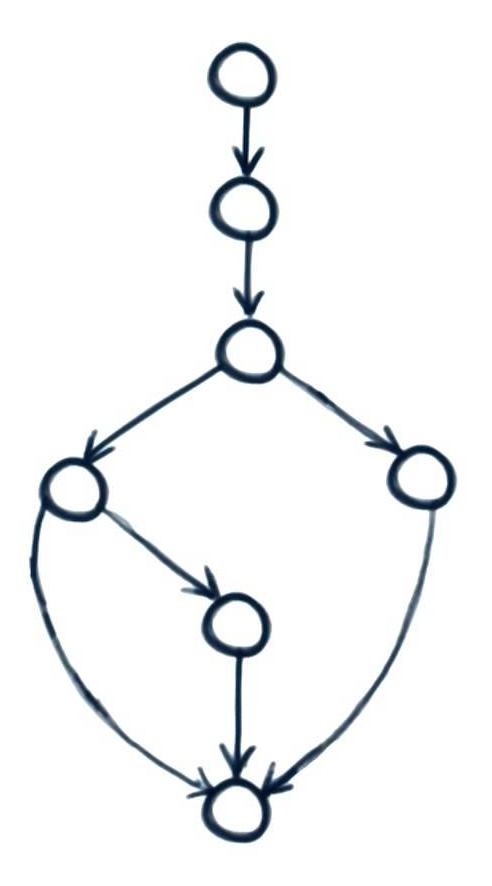
\includegraphics[scale=0.25]{controlflow}
	\end{textblock*}
	
	\begin{textblock*}{8cm}(4.5cm,1.7cm)
		\begin{itemize}
			\item \textbf{Sanitization problem} \\
					\only<2->{
							{\hspace{1cm}\color[rgb]{1,1,1} \texttt{b := a $\oplus$ a}}
					}
			\item<3-> Pure dynamic taint analysis considers \textbf{data flows}... \newline
		  ...but it ignores \textbf{control-flows} \newline
					{\color[rgb]{1,1,1}
						\texttt{x = get\_input(src)} \\
						\texttt{if x == 1 then } \\
							{\hspace{0.7cm}\texttt{y = 1}\\}
						\texttt{...} \\
						\texttt{goto y}
					}
			\item<4-> What about different security policies for different I/O channels? \newline
			\only<5->{$\rightarrow$ \textbf{Static analysis}}
		\end{itemize}
	\end{textblock*}
\end{frame}

\section{Forward Symbolic Execution}
\begin{frame}[fragile]
	\frametitle{Forward Symbolic Execution}
	\begin{itemize}
		\item We can reason about the behavior of a program using the logic...
		\item ... and it is \textbf{conceptually} a very simple process
	\end{itemize}
	\lstset{language=C++,
		basicstyle=\color{white}\ttfamily,
		commentstyle=\color{green}\ttfamily,
		%		numbers=left
	}
	\begin{lstlisting}
	x := 2 * get_input(src)
	if x - 5 == 14 then goto 3 else goto 4
	// line 3: catastrophic failure
	// line 4: normal behaviour
	\end{lstlisting}
	\only<2->{
		\begin{itemize}
			\item \texttt{get\_input(src)} now returns a \textbf{symbol} instead of a concrete value
			\item But now expressions \textbf{cannot} be fully evaluated to a concrete value
		\end{itemize}
	}
\end{frame}
\begin{frame}
	\frametitle{Path Selection and Performance}
	\begin{itemize}
		\item For each conditional jump we must decide what path to follow first
		\begin{itemize}
			\item But some path may never terminate
		\end{itemize}
		\item Exponential blowup due to branches
	\end{itemize}
	\centering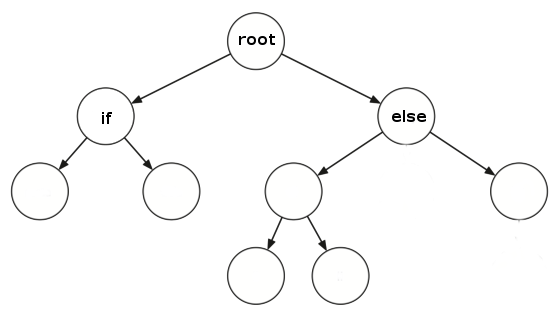
\includegraphics[scale=0.85]{tree}
\end{frame}

\section{Conclusions}
\begin{frame}
	\frametitle{A small comparison}
	\only<1>{
		\begin{textblock*}{5cm}(0cm,4cm)
			\fontsize{20pt}{12pt}\selectfont\centering
			Dynamic\\Taint\\Analysis
		\end{textblock*}
		
		\begin{textblock*}{5cm}(4cm,4cm)
			\centering
			\fontsize{15pt}{12pt}\selectfont
			? \\
			\fontsize{30pt}{12pt}\selectfont
			$\subseteq$ \\
			$\supseteq$
		\end{textblock*}
		
		\begin{textblock*}{5cm}(8cm,4cm)
			\fontsize{20pt}{12pt}\selectfont\centering
			Forward\\Symbolic\\Execution
		\end{textblock*}
	}
	\only<2>{
		\vspace{-1cm}
		\centering
		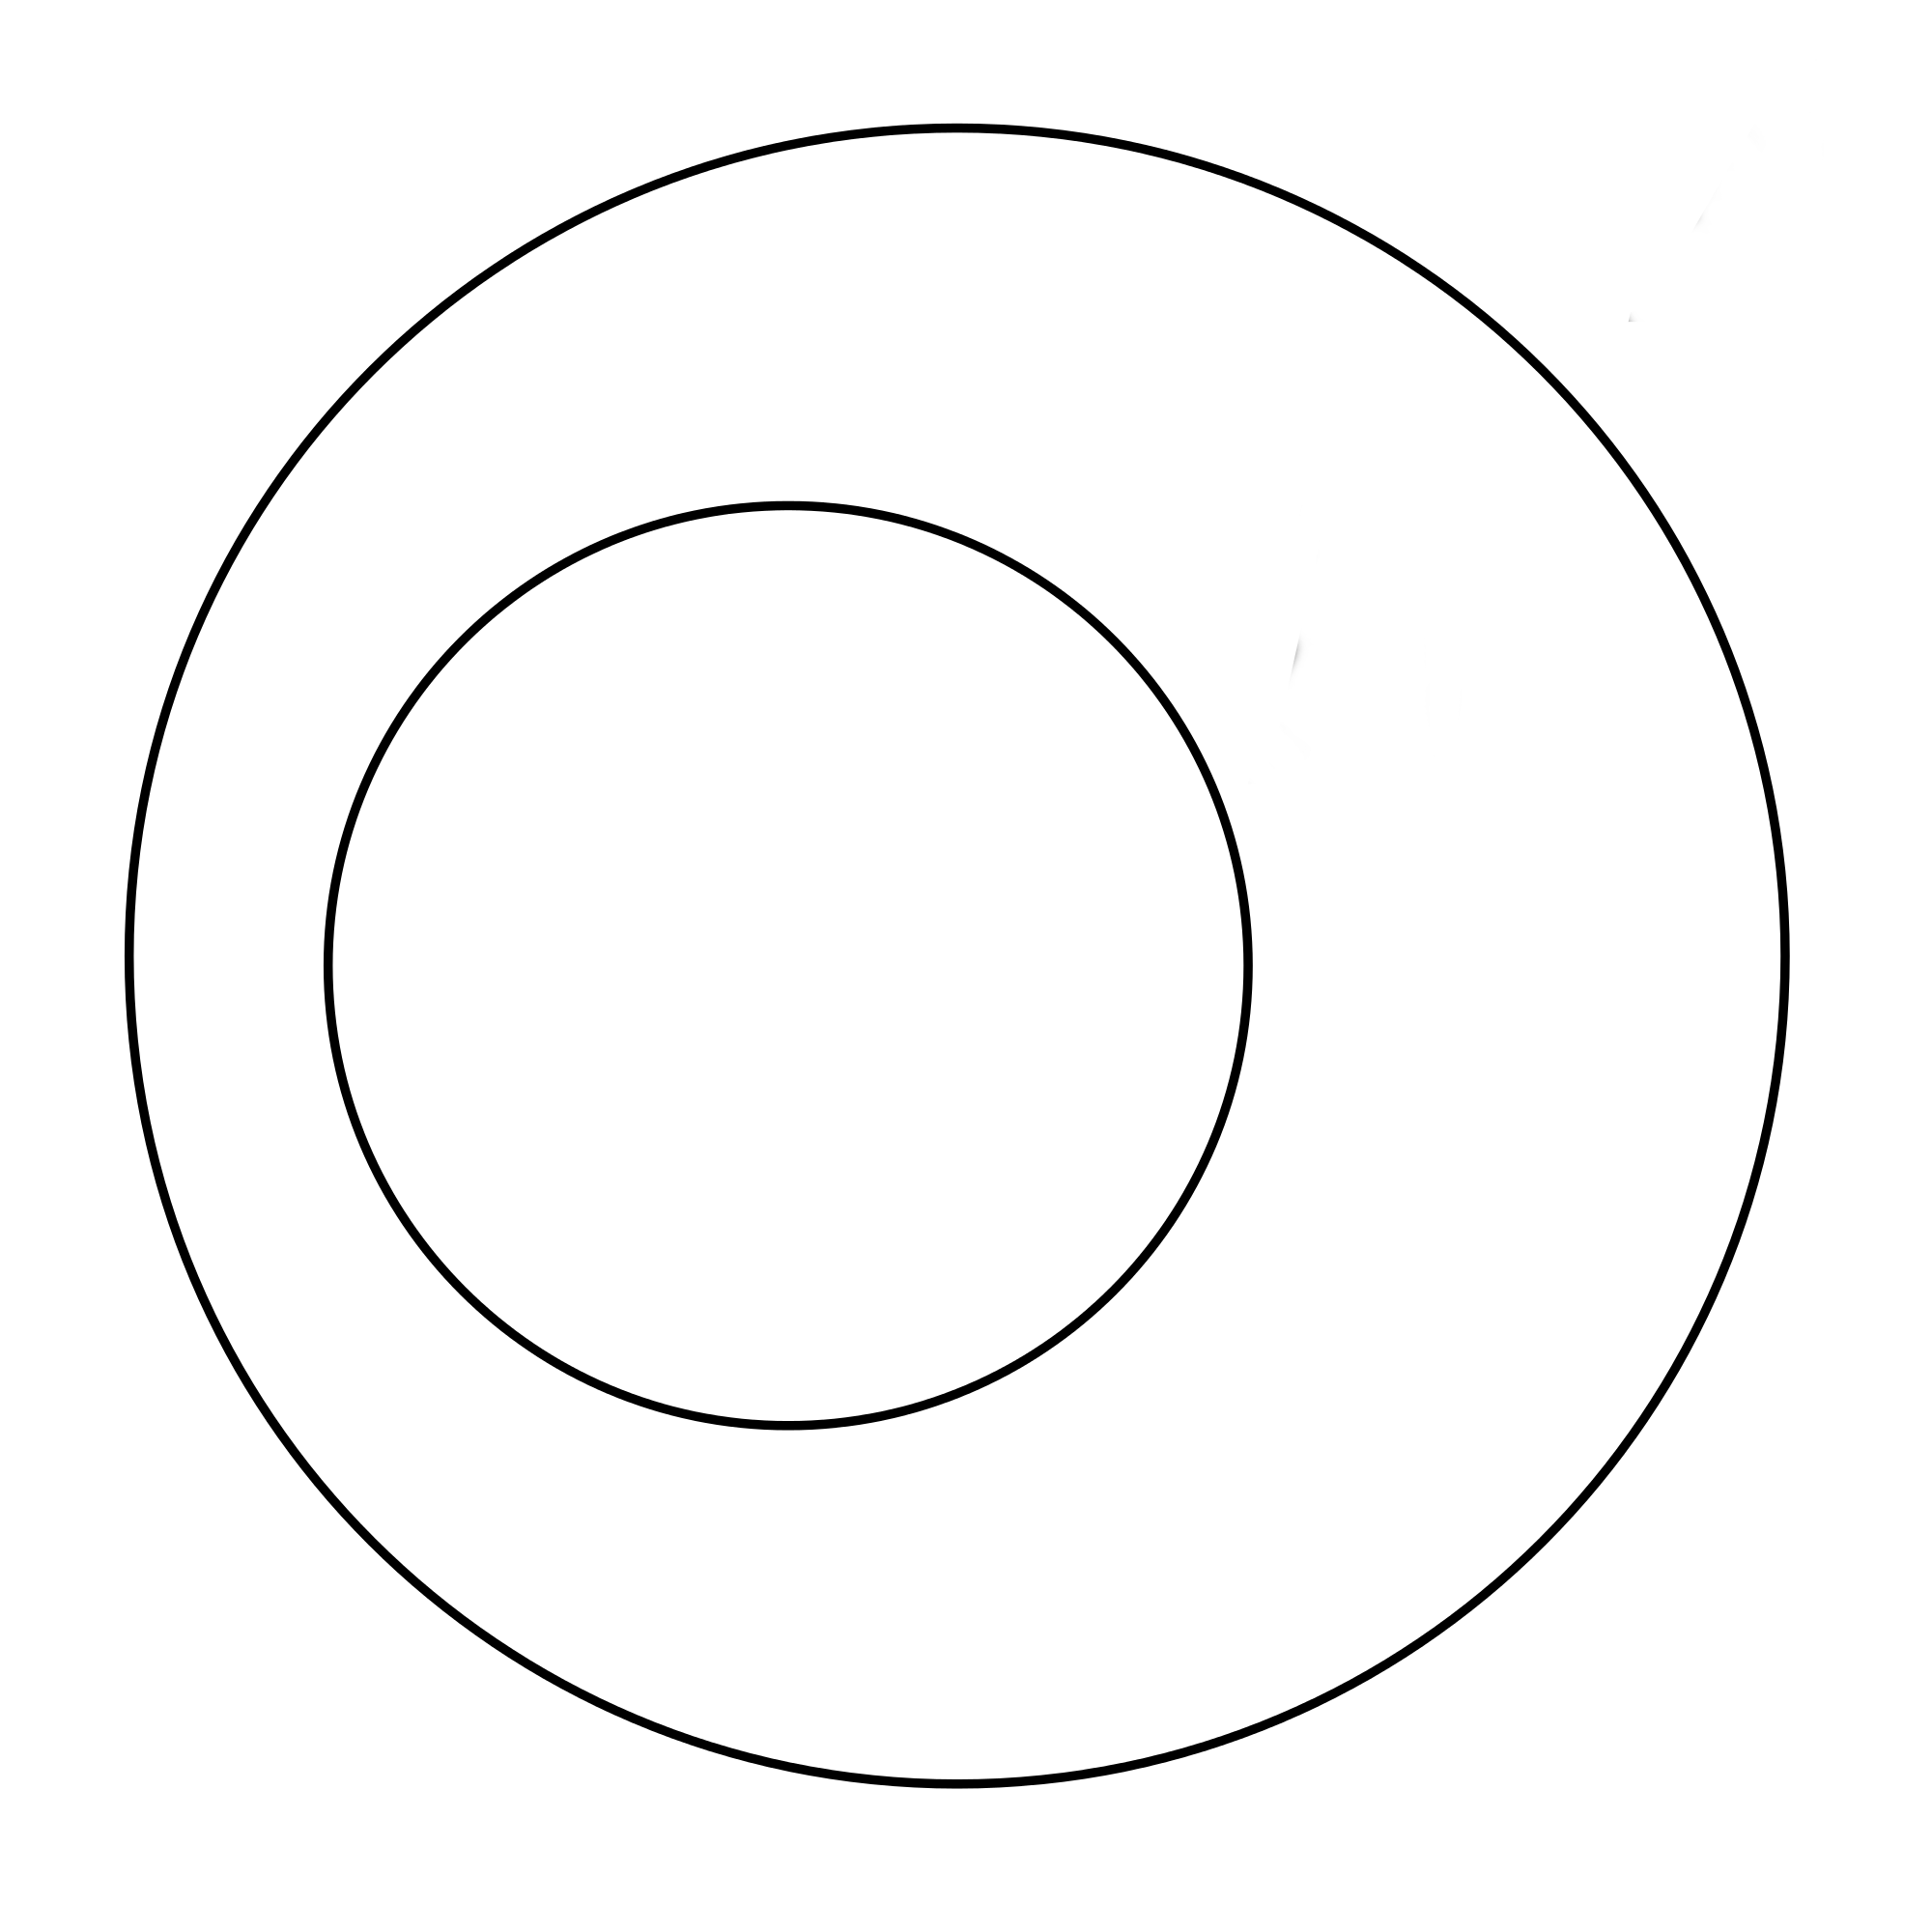
\includegraphics[scale=0.1]{sets} \\
		Dynamic taint analysis analyzes only \textit{\textbf{feasible}} paths
		\fontsize{18pt}{12pt}\selectfont
		\begin{textblock*}{5cm}(3cm,3.6cm)
			$\mathcal{DTA}$
		\end{textblock*}
		\begin{textblock*}{5cm}(4.6cm,2cm)
			$\mathcal{FSE}$
		\end{textblock*}
	}
\end{frame}
\section{Conclusions}
\subsection{Comparison}
In my opinion, symbolic execution uses a kind of taint analysis to construct path constraints. Symbolic execution also employs an SMT solver to generate concrete values for variables and/or inputs, such that a certain path constraint is satisfied. Since taint analysis does not employ an SMT solver, I would say it is not a kind of symbolic execution.

Furthermore, dynamic analysis can also reason about \textit{feasible} path, while symbolic execution builds constraint and reasons about the whole program by reducing it in the domain of logic.

Thus, in my opinion, taint analysis is a \textbf{subset} of symbolic execution.

\subsection{Last things}
The number of security applications utilizing these two techniques is enormous. Example security research areas employing either dynamic taint analysis, forward symbolic execution, or a mix of the two, are the following:
\begin{itemize}
	\item \textbf{Unknown Vulnerability Detection}: Dynamic taint analysis can look for misuses of user input during an execution. For example, dynamic taint analysis can be used to prevent code injection attacks by monitoring whether user input is executed;
	\item \textbf{Malware Analysis}: Taint analysis and forward symbolic execution are used to analyze how information flows through a malware binary, explore trigger-based behavior and detect emulators;
	\item \textbf{Test Case Generation}: Taint analysis and forward symbolic execution are used to automatically generate inputs to test programs, and can generate inputs that cause two implementations of the same protocol to behave differently;
	\item \textbf{Automatic Network Protocol Understanding}: Dynamic taint analysis has been used to automatically understand the behavior of network protocols.
\end{itemize}

However, recalling the limitations and the problems with both analysis I would say that they have to be used carefully. Their effectiveness depends on the specific application.



\appendix
\makethanks
\newcommand{\turnOffNumbers}{} %hide frame numbers in footer
\begin{frame}[noframenumbering]
	\frametitle{SimpIL Grammar}
	\vspace{-0.5cm}
	\only<1>{
		\begin{center}
			\hspace{1.3cm}
			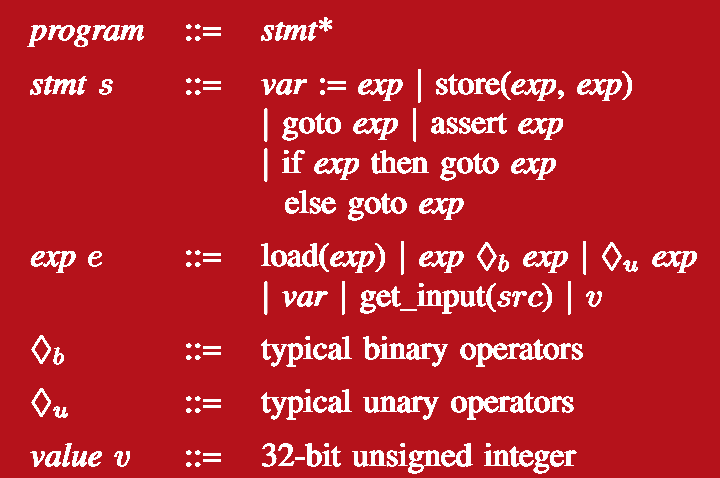
\includegraphics[scale=0.30]{SimpIL}
		\end{center}
	}
\end{frame}
\begin{frame}[noframenumbering]
	\frametitle{SimpIL Operational Semantic}
	\begin{itemize}		
		\item \textbf{Each} statement rule of the operational semantic is like:		
	\end{itemize}		
	\begin{prooftree}		
		\AxiomC{computation}		
		\UnaryInfC{$\textless$current state$\textgreater$, stmt $\rightarrow$ $\textless$end state$\textgreater$, stmt’}		
	\end{prooftree}		
	\begin{itemize}		
		\item The \texttt{state} is composed of: \newline		
	\begin{minipage}{0.5\textwidth}		
		\begin{itemize}		
			\item Program statements (\bm{$\sum$})		
			\item Current memory state (\bm{$\mu$})		
			\item Current values for variables (\bm{$\Delta$})		
		\end{itemize}		
	\end{minipage}		
	\begin{minipage}{0.4\textwidth}		
		\begin{itemize}		
			\item Program counter (\textbf{\textit{pc}})		
			\item Current statement (\textit{\textbf{i}})		
		\end{itemize}		
	\end{minipage}		
\end{itemize}
\end{frame}
\begin{frame}
	\frametitle{Memory Address Problems}
	\begin{itemize}
		\item What are we supposed to do if a referenced address is derived from user input?
		\begin{itemize}
			\item \texttt{LOAD}, \texttt{STORE} $\rightarrow$ \textbf{Symbolic Memory Address}
			\item \texttt{GOTO} $\rightarrow$ \textbf{Symbolic Jumps}
		\end{itemize}
		\item Solutions
		\begin{itemize}
			\item Concolic testing
			\item SMT (\textbf{S}atisfiability \textbf{M}odulo \textbf{T}heories) solvers
			\item Static and alias analysis
		\end{itemize}
	\end{itemize}
\end{frame}
\end{document}
